The results of the experiments using different training sample sizes for the SVM classifiers are displayed in table \ref{tab:svm}. As more training samples are used to train the SVM classifier performance increases, which is expected for supervised classification. When the training set size reaches more than 75 images per class the classifiers overfit due to noise in the data which results in a decrease in performance.
  
\begin{table}[H]
\begin{tabular}{|c|ccccc|}
\hline
\textbf{Training set size} & \textbf{AP Airplanes} & \textbf{AP Cars} & \textbf{AP Faces} & \textbf{AP Motorbikes} & \textbf{MAP}\\
\hline
30 & 0.6647 & 0.8898 & 0.3772 & 0.5184& 0.6125\\
50 & 0.6484 & 0.9096 & 0.8780 & 0.6627 & 0.7747\\
70 & 0.6531 & 0.8441 & 0.7156 & 0.7590 & 0.7429\\
75 & 0.6447 & 0.9053 & 0.9510 & 0.7516 & 0.8132\\
90 & 0.6426 & 0.8697 & 0.5227 & 0.6963 & 0.6828\\
\hline
\end{tabular}
\caption{Effect number of training set size (per class) for SVM, Sift type: dense, Color space: opponent}
\label{tab:svm}
\end{table}

A surprising result is that the airplane and car classifiers obtain a stable performance for the different training set sizes. This is clearly shown in Figure \ref{fig:svm}. A possible explanation is that the airplane and car images have little noise (which can cause overfitting of the model) and can be contained in simple feature descriptions as the model shows to be less prone to underfit. The images in the dataset for each of these classes are taken from the same angle and the form of the objects are more similar than faces or motorbikes, which result in a more stable performance.

\begin{figure}[H]
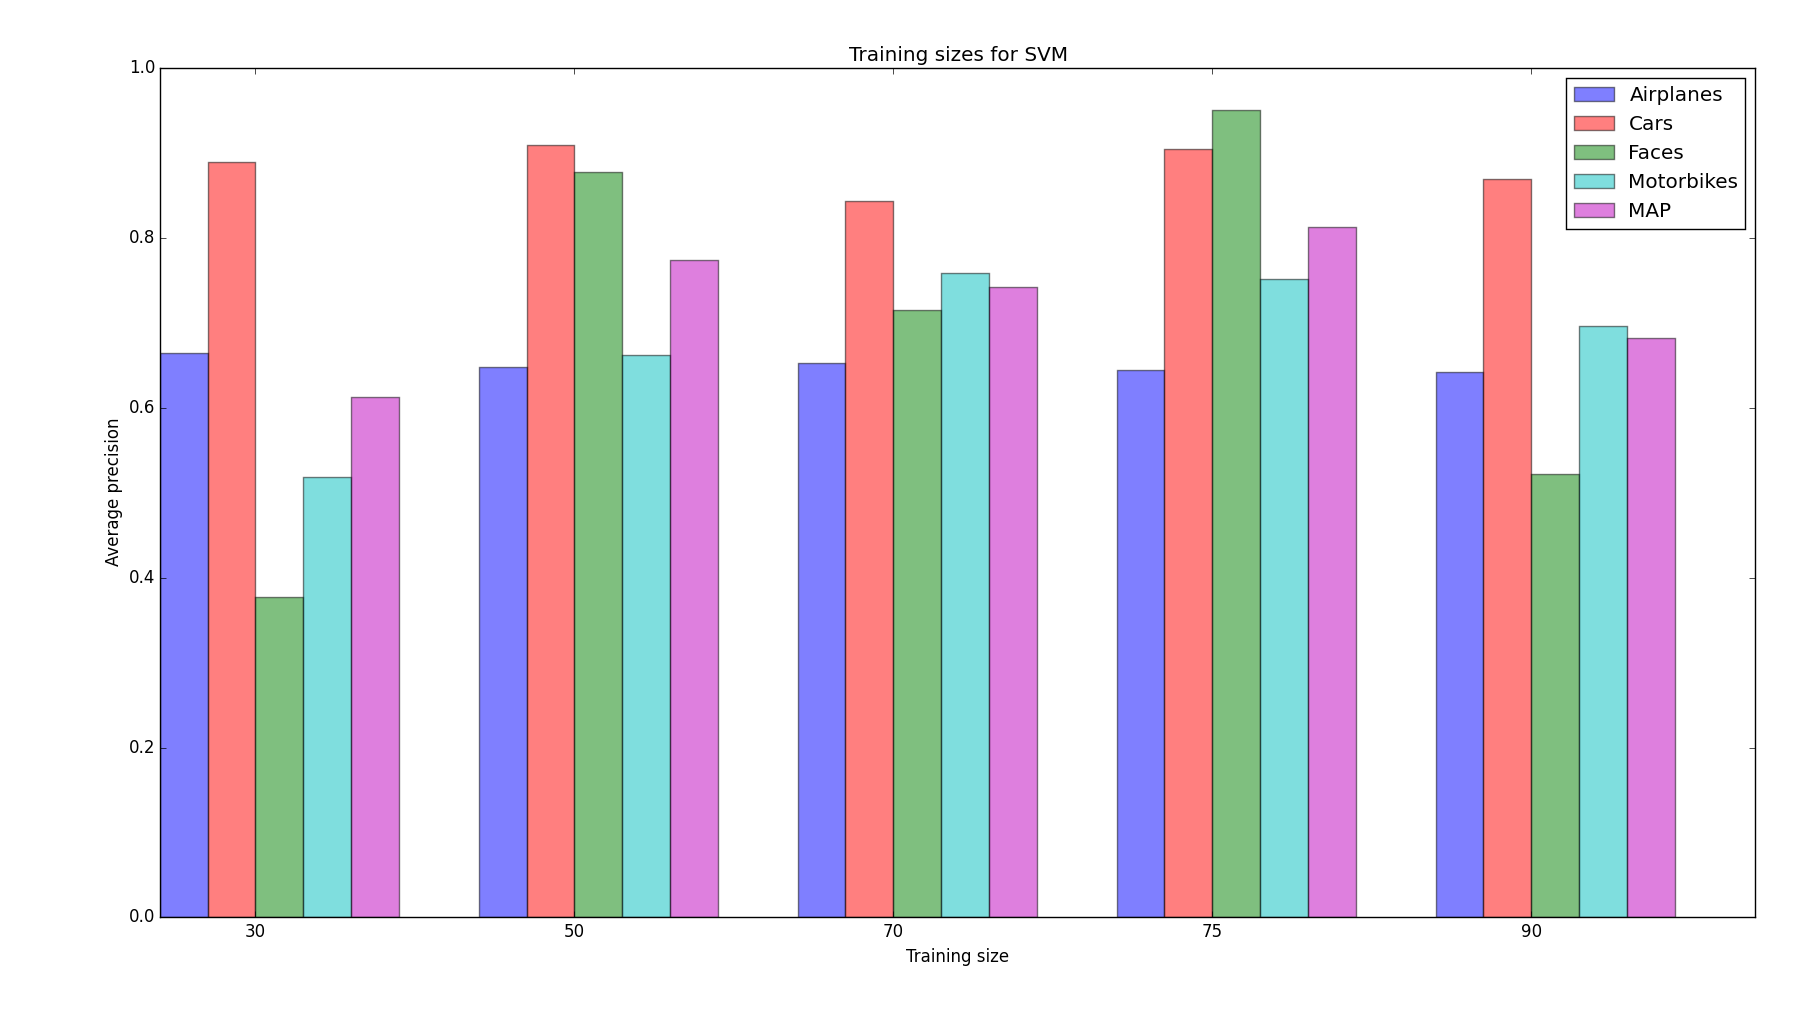
\includegraphics[width=\textwidth]{../plots/training_size_SVM}
\caption{Effect of training size for SVMs on AP}
\label{fig:svm}
\end{figure}
